% Paper-style snapshot of the candidate screen.
% The growing full dissertation draft lives in:
%   docs/dissertation/main.tex
% Prefer new writing there; keep this file as a compact report extract.

\documentclass[11pt,reprint,aps,prl,floatfix,secnumarabic]{revtex4-2}

\usepackage[T1]{fontenc}
\usepackage{amsmath}
\usepackage{amssymb}
\usepackage{booktabs}
\usepackage{graphicx}
\usepackage[hidelinks]{hyperref}
\usepackage{microtype}
\microtypesetup{expansion=false}

\graphicspath{{figures/full_candidate_perturbation/}}
\raggedbottom

\begin{document}

\title{Exploring Candidate RNN Perturbations for
Psilocybin-Related Working-Memory Effects}

\author{Bob Rice}
\affiliation{University of Nottingham}

\maketitle

\section{Methods}

\subsection{Fixation-gated circular delayed-response task}

Each circular-task trial comprised pre-cue fixation, a circular cue, a silent
memory delay, and a response period. Stimulus angle
$\theta\in[0,2\pi)$ was encoded over 32 evenly spaced preferred angles
$\mu_j$ as
\begin{equation}
 c_j(\theta)=\exp\{\kappa[\cos(\theta-\mu_j)-1]\},\qquad \kappa=8.
\end{equation}
The fixation input and output remained high until the response cue. Circular
outputs were deliberately silent before response and then reported the
remembered angle. Pre-cue and cue durations varied during training; evaluation
used clean delays of 10, 20, 40, and 80 model steps. A separate delay-20
condition inserted a five-step irrelevant circular cue midway through the
delay. Training sampled one clean and one distractor-present homogeneous batch
exactly once per shuffled two-batch block. Distractor filtering was therefore a
learned property of the evaluated networks rather than an out-of-distribution
challenge.

\subsection{Context-cued N-back task}

The N-back task presented 20 sequential items drawn from six stimulus
identities. Two context channels instructed either
0-back or 2-back behaviour. In 0-back, the network classified whether the
current item matched a fixed target identity. In 2-back, it classified whether
the current item matched the item presented two positions previously.
Sequences contained six matches; the 2-back generator additionally controlled
one-back lures. The first two items were excluded from scored outcomes. The
output consisted of match and non-match logits.

\subsection{Recurrent networks and checkpoint replication}

Both task families used 64-unit \texttt{tanh} recurrent networks with
$dt=20$, $\tau=100$, and $\alpha=dt/\tau=0.2$. The native update was
\begin{align}
 z_t &= W_{\mathrm{in}}x_t+b_{\mathrm{in}}
      +W_{\mathrm{rec}}h_{t-1}+b_{\mathrm{rec}},\\
 h_t &= \tanh\!\left[(1-\alpha)h_{t-1}+\alpha z_t\right].
 \label{eq:native}
\end{align}
The circular model had 33 inputs and outputs: 32 tuned channels plus
fixation. The N-back model had six stimulus inputs, two rule-context inputs,
and two outputs. Circular networks were trained for 4,000 Adam updates
(learning rate $10^{-3}$, batch size 64) with weighted fixation and
response loss on a balanced clean/distractor mixture. Training used input noise
SD 0.01, recurrent noise SD 0.05, and gradient clipping at 1.0; all learned
weights were then frozen before perturbation. Six circular seeds were trained;
five met
preconfigured competence limits (clean mean error $\le10^\circ$, distractor
mean error $\le15^\circ$, fixation accuracy $\ge0.90$) and were retained
(seeds 20260731, 20260732, 20260733, 20260735, and 20260736). Seed 20260734
exceeded those limits (clean $15.75^\circ$, distractor $17.46^\circ$) and was
excluded before the perturbation screen. The ten N-back checkpoints
(seeds 20260912--20260921) were drawn from a competence-screened pool trained
with staged 0-back then 2-back curriculum under Adam (learning rate $10^{-3}$).
Final N-back retention required accuracy $\ge0.95$, discriminability
(hit rate minus false-alarm rate) $\ge0.90$, and 2-back lure accuracy
$\ge0.90$ on both loads; stage-1 0-back acquisition used stricter gates
(accuracy $\ge0.98$, discriminability $\ge0.95$) before 2-back training.
A checkpoint is one independently trained network with frozen weights,
identified by its random seed. Independently trained checkpoint, not trial or
technical replicate, was the replication unit.

These gates are operational competence thresholds, not fitted human effect
sizes. Chance circular error is of order $90^\circ$, so clean $\le10^\circ$
requires unambiguous angle memory while remaining softer than the few-degree
errors typical of retained seeds; distractor $\le15^\circ$ allows a modest
filtering cost without accepting near-failure. Fixation $\ge0.90$ keeps the
network in a reliable go regime so latency contrasts are not confounded by
fixation collapse. N-back gates likewise demand near-ceiling fixed-target
performance, clearly above-chance updating, and lure resistance, so load
contrasts reflect selective updating cost rather than a weak baseline.

\subsection{Candidate perturbations}

We evaluated seven single-operator families against each checkpoint's native
baseline (Table~\ref{tab:perturbations}). Operators are competing computational
interventions motivated by, but not equated with, psychedelic or working-memory
mechanisms. Because the native update applies $\tanh$ after mixing drive with
carried state, no operator is an exact biological response-gain map; each is an
explicit RNN translation. Unless noted, every non-neutral operator was applied
at every timestep of the full frozen forward pass for the entire trial or
sequence; learned weights were never updated. The only timed exception is P3b,
which is confined to the irrelevant circular-cue window. Write
$z_t^{\mathrm{w}}=W_{\mathrm{in}}x_t+W_{\mathrm{rec}}h_{t-1}$ for the
weight-derived drive. Symbols are shared across perturbations:
$x_t$ is input, $h_t$ hidden state, and $z_t$ pre-activation drive at time
$t$; $W_{\mathrm{in}}$ and $W_{\mathrm{rec}}$ are input and recurrent weights;
$b_{\mathrm{in}}$ and $b_{\mathrm{rec}}$ are biases; and $\alpha=dt/\tau$ is
the native leak factor. In P3a/P3b, $x_t^{\mathrm{stim}}$ and
$x_t^{\mathrm{ctrl}}$ denote stimulus versus fixation/rule-control channels,
with matching input submatrices $W_{\mathrm{in}}^{\mathrm{stim}}$ and
$W_{\mathrm{in}}^{\mathrm{ctrl}}$. Scalar $g$ denotes uniform gain, vector
$\mathbf{g}$ fixed unit-wise gain (P2), $\varepsilon_t\sim\mathcal{N}(0,I)$
Gaussian noise scaled by $\sigma$ (P5), $p$ persistence scale (P6), and $s$
timescale factor with derived $\alpha'$ (P7). Unless noted, learned biases
stay outside multiplicative gains.

\subsubsection{P1 Synaptic-drive gain}
Herzog et al.\ operationalised 5-HT2A effects as response gain on synaptic
current inside a nonlinearity \cite{herzog2023}; REBUS likewise links altered
precision to postsynaptic gain \cite{carhartharris2019}. In this CTRNN the
closest available analogue multiplies weight-derived drive while leaving
biases unscaled:
\begin{equation}
 h_t=\tanh\!\left[
 (1-\alpha)h_{t-1}+\alpha\bigl(g z_t^{\mathrm{w}}+b_{\mathrm{in}}+b_{\mathrm{rec}}\bigr)
 \right].
 \label{eq:p1}
\end{equation}
This is synaptic-drive gain, not an exact $F$--$I$ slope change and not a pure
carried-state manipulation.

\subsubsection{P2 Heterogeneous drive gain}
Receptor-density dependence in Herzog et al.\ implies spatially nonuniform gain
rather than one global scalar \cite{herzog2023}. We therefore replaced $g$ by a
fixed positive unit-wise vector $\mathbf{g}$ drawn from a log-normal
distribution and normalised to population mean one:
\begin{equation}
 h_t=\tanh\!\left[
 (1-\alpha)h_{t-1}+\alpha\bigl(\mathbf{g}\odot z_t^{\mathrm{w}}+b_{\mathrm{in}}+b_{\mathrm{rec}}\bigr)
 \right].
 \label{eq:p2}
\end{equation}
Three fixed vectors were treated as technical replicates and averaged within
checkpoint; they are not independent trained seeds.

\subsubsection{P3a Sensory-input gain}
REBUS predicts increased influence of afferent or bottom-up signals when
high-level precision is relaxed \cite{carhartharris2019}. As a task-level
translation, only stimulus-channel input weights were scaled, leaving fixation
or rule-context channels unchanged:
\begin{equation}
\begin{aligned}
 z_t^{\mathrm{in}} &=
 g\,W_{\mathrm{in}}^{\mathrm{stim}}x_t^{\mathrm{stim}}
 +W_{\mathrm{in}}^{\mathrm{ctrl}}x_t^{\mathrm{ctrl}}
 +b_{\mathrm{in}},\\
 h_t &= \tanh\bigl[(1-\alpha)h_{t-1}
 +\alpha(z_t^{\mathrm{in}}+W_{\mathrm{rec}}h_{t-1}+b_{\mathrm{rec}})\bigr].
\end{aligned}
 \label{eq:p3a}
\end{equation}
This tests sensory sensitivity, not receptor-mapped response gain.

\subsubsection{P3b Distractor-window gain}
Carter et al.\ reported impaired multiple-object tracking with comparatively
spared spatial working-memory span and proposed weakened filtering of irrelevant
information \cite{carter2005}. P3b applies Eq.~\eqref{eq:p3a} only during the
irrelevant circular cue and is therefore a circular-task manipulation check
rather than a complete cross-task mechanism candidate.

\subsubsection{P4 Recurrent gain}
Recurrent excitation is a canonical substrate of delay-period maintenance
\cite{wang2013nmda}. To separate recurrent weighting from sensory drive we
scaled only the recurrent weight contribution:
\begin{equation}
\begin{aligned}
 z_t^{(4)} &=
 W_{\mathrm{in}}x_t+b_{\mathrm{in}}
 +g W_{\mathrm{rec}}h_{t-1}+b_{\mathrm{rec}},\\
 h_t &= \tanh\bigl[(1-\alpha)h_{t-1}+\alpha z_t^{(4)}\bigr].
\end{aligned}
 \label{eq:p4}
\end{equation}
Recurrent bias remained outside the gain. P4 is a mechanistic contrast within
the trained RNN, not a direct REBUS or 5-HT2A claim.

\subsubsection{P5 Gaussian state noise}
Independent Gaussian noise is retained as a generic disruption control against
which selective signatures must later be shown to exceed nonspecific damage.
Noise would be added to the pre-activation,
\begin{equation}
 h_t=\tanh\!\left[
 (1-\alpha)h_{t-1}+\alpha z_t+\sigma\varepsilon_t
 \right],
 \quad \varepsilon_t\sim\mathcal{N}(0,I),
 \label{eq:p5}
\end{equation}
but P5 was not evaluated in this candidate-only screen.

\subsubsection{P6 State persistence}
Trained working-memory RNNs can store information along slow latent manifolds
\cite{ghazizadeh2021}, while neurophysiological evidence links NMDA-dependent
persistent firing to working-memory maintenance \cite{wang2013nmda}. P6 asks
whether weakening retention of the carried state, without rescaling incoming
drive, can produce selective behavioural costs. The update is asymmetric:
\begin{equation}
 h_t=\tanh\!\left[p(1-\alpha)h_{t-1}+\alpha z_t\right],
 \label{eq:persistence}
\end{equation}
where $p$ is the persistence scale. This is an operational RNN intervention,
not a pre-specified biological mapping from psilocybin to reduced persistence.

\subsubsection{P7 Conserved effective time constant}
To test whether P6 effects are merely those of any timescale change, P7
rescales the leaky-integrator coefficients while preserving their sum. With
timescale factor $s$,
\begin{equation}
 \alpha'=\min(\alpha/s,1),\qquad
 h_t=\tanh\!\left[(1-\alpha')h_{t-1}+\alpha'z_t\right].
 \label{eq:p7}
\end{equation}
Thus $s>1$ slows the effective timescale and $s<1$ speeds it. Within the
evaluated grid, $\alpha/s<1$, so the minimum was inactive. P7 is a
mechanistic control for conserved timescale change, not a psychedelic
parameter claim.

\begin{table*}[t]
\caption{\textbf{Candidate perturbations and fixed evaluation grids.}
Neutral settings reproduce the native forward pass. Distractor-window gain was
defined only for the circular distractor condition; all other operators except
P5 were evaluated in both task families. P5 is listed as the planned generic
control but was not part of this screen.}
\label{tab:perturbations}
\centering
\begin{tabular}{llll}
\toprule
ID & Perturbation & Computational intervention & Strengths \\
\midrule
P1 & Synaptic-drive gain & Scalar gain on input and recurrent weight drive
& 0.90, 0.95, 1.00, 1.05, 1.10 \\
P2 & Heterogeneous drive gain & Fixed mean-one unit-wise log-normal gain
& log-SD 0.00, 0.10, 0.20, 0.30 \\
P3a & Sensory-input gain & Gain on stimulus-channel input contribution
& 0.80, 0.90, 1.00, 1.10, 1.20 \\
P3b & Distractor-window gain & P3a restricted to irrelevant cue window
& 1.00, 1.10, 1.25, 1.50 \\
P4 & Recurrent gain & Scalar gain on recurrent weight contribution
& 0.90, 0.95, 1.00, 1.05, 1.10 \\
P5 & Gaussian state noise & Additive pre-activation noise (not screened)
& not evaluated here \\
P6 & State persistence & Scale $p$ on carried-state coefficient
& 0.90, 0.95, 1.00, 1.05, 1.10 \\
P7 & Effective time constant & Conserved update with $\alpha'=\min(\alpha/s,1)$
& 0.80, 0.90, 1.00, 1.10, 1.25 \\
\bottomrule
\end{tabular}
\end{table*}

\subsection{Evaluation and behavioural signature}

The evaluated contrasts were qualitative model analogues of selected acute
human findings rather than fitted human effect sizes. A stronger acute effect
on response time than accuracy motivated slowing with relative preservation
\cite{yousefi2025}; selective 2-back impairment relative to 0-back motivated
the N-back load contrast \cite{barrett2018}; and impaired multiple-object
tracking with comparatively spared spatial span motivated the filtering
contrast \cite{carter2005}. Delay selectivity was retained as supporting
mechanistic evidence rather than a scored human-signature requirement.

Each circular checkpoint, operator, strength, condition, and delay used 1,024
trials. Each N-back checkpoint, operator, strength, and load used 1,024
20-item sequences. Native and perturbed evaluations reused identical generated
task samples within checkpoint and cell.

Circular response accuracy was mean absolute angular error. Post-cue settling
was the first response step at which angular error was below $15^\circ$ and
population-vector amplitude exceeded 50\% of the native reference amplitude.
Trials that did not settle were capped at the 25-step response duration,
yielding restricted mean settling time. Settling was interpreted only when
fixation accuracy was at least 0.90 and at least 80\% of trials settled.
The $15^\circ$ settling threshold is a coarse ``pointing near the target''
latency criterion, distinct from the continuous accuracy metric; the
half-native amplitude rule excludes weak or collapsed population bumps; and
the 80\% settled floor marks latency invalid when most trials never settle.
``Slowing with preservation'' required a positive settling change at clean
delay 20 while proportional angular-error impairment remained at or below
0.20. That 20\% relative-error ceiling encodes selective slowing without large
accuracy loss: small clean costs remain allowed, but wholesale damage fails
the preservation half of the signature.

For circular condition $c$, proportional impairment was
\begin{equation}
 I_c=\frac{E_{\mathrm{perturbed},c}-E_{\mathrm{native},c}}
 {E_{\mathrm{native},c}},
\end{equation}
where $E$ is mean angular error. Delay selectivity was
$I_{\mathrm{delay\,80}}-I_{\mathrm{delay\,10}}$; distractor selectivity was
$I_{\mathrm{distractor\,20}}-I_{\mathrm{clean\,20}}$.

N-back discriminability was $D=H-F$, where $H$ and $F$ are hit and false-alarm
rates. Condition-normalised impairment was
\begin{equation}
 J_c=\frac{D_{\mathrm{native},c}-D_{\mathrm{perturbed},c}}
 {D_{\mathrm{native},c}},
\end{equation}
and load selectivity was $J_{\mathrm{2back}}-J_{\mathrm{0back}}$. Positive
values indicate disproportionate high-load impairment.

The analysis was descriptive. For each operator-strength setting we reported
the checkpoint mean, SD, and a student $t$ 95\% interval across seeds, together
with the fraction of seeds in the predicted direction. A setting met the
complete descriptive pattern when the mean slowing-with-preservation,
distractor, and N-back load contrasts were positive and at least a simple
majority of checkpoints agreed on each (three of five circular; six of ten
N-back); delay selectivity was supporting evidence only. That majority rule is
implemented in the summary code; it was not restated as a numeric threshold in
the 1,024-trial preregistration text. Cross-operator comparisons are uncontrolled
for overall perturbation magnitude, so a near-miss may fail because of strength
selection as well as mechanism. No participant-level inference, confirmatory
$p$ values, or multiple-comparison claims were made.

Persistence 0.95 had been nominated by an earlier three-checkpoint exploratory
pilot. The present analysis is therefore a retest on newly trained circular
checkpoints and an expansion of the partially overlapping N-back evaluation,
not a fresh blind screen. Three of the ten N-back checkpoints (seeds
20260912--20260914) contributed to the nomination pilot.

\section{Results}

\subsection{One descriptive profile met the complete majority pattern}

Across the 23 non-neutral shared operator-strength profiles evaluated on the
distractor-trained circular family and the ten N-back checkpoints, only
persistence $0.95$ met the complete descriptive majority pattern
(Fig.~\ref{fig:screen}). It showed slowing with preservation, long-delay
selectivity, and distractor selectivity in four of five circular checkpoints,
together with load selectivity in all ten N-back checkpoints. Mean circular
delay selectivity was $0.089$ and mean distractor selectivity $0.015$; N-back
load selectivity was $0.250$. Neutral settings returned zero contrast. Other
perturbations often reproduced one or two components, but not the full
combination.

\begin{figure*}[t]
  \centering
  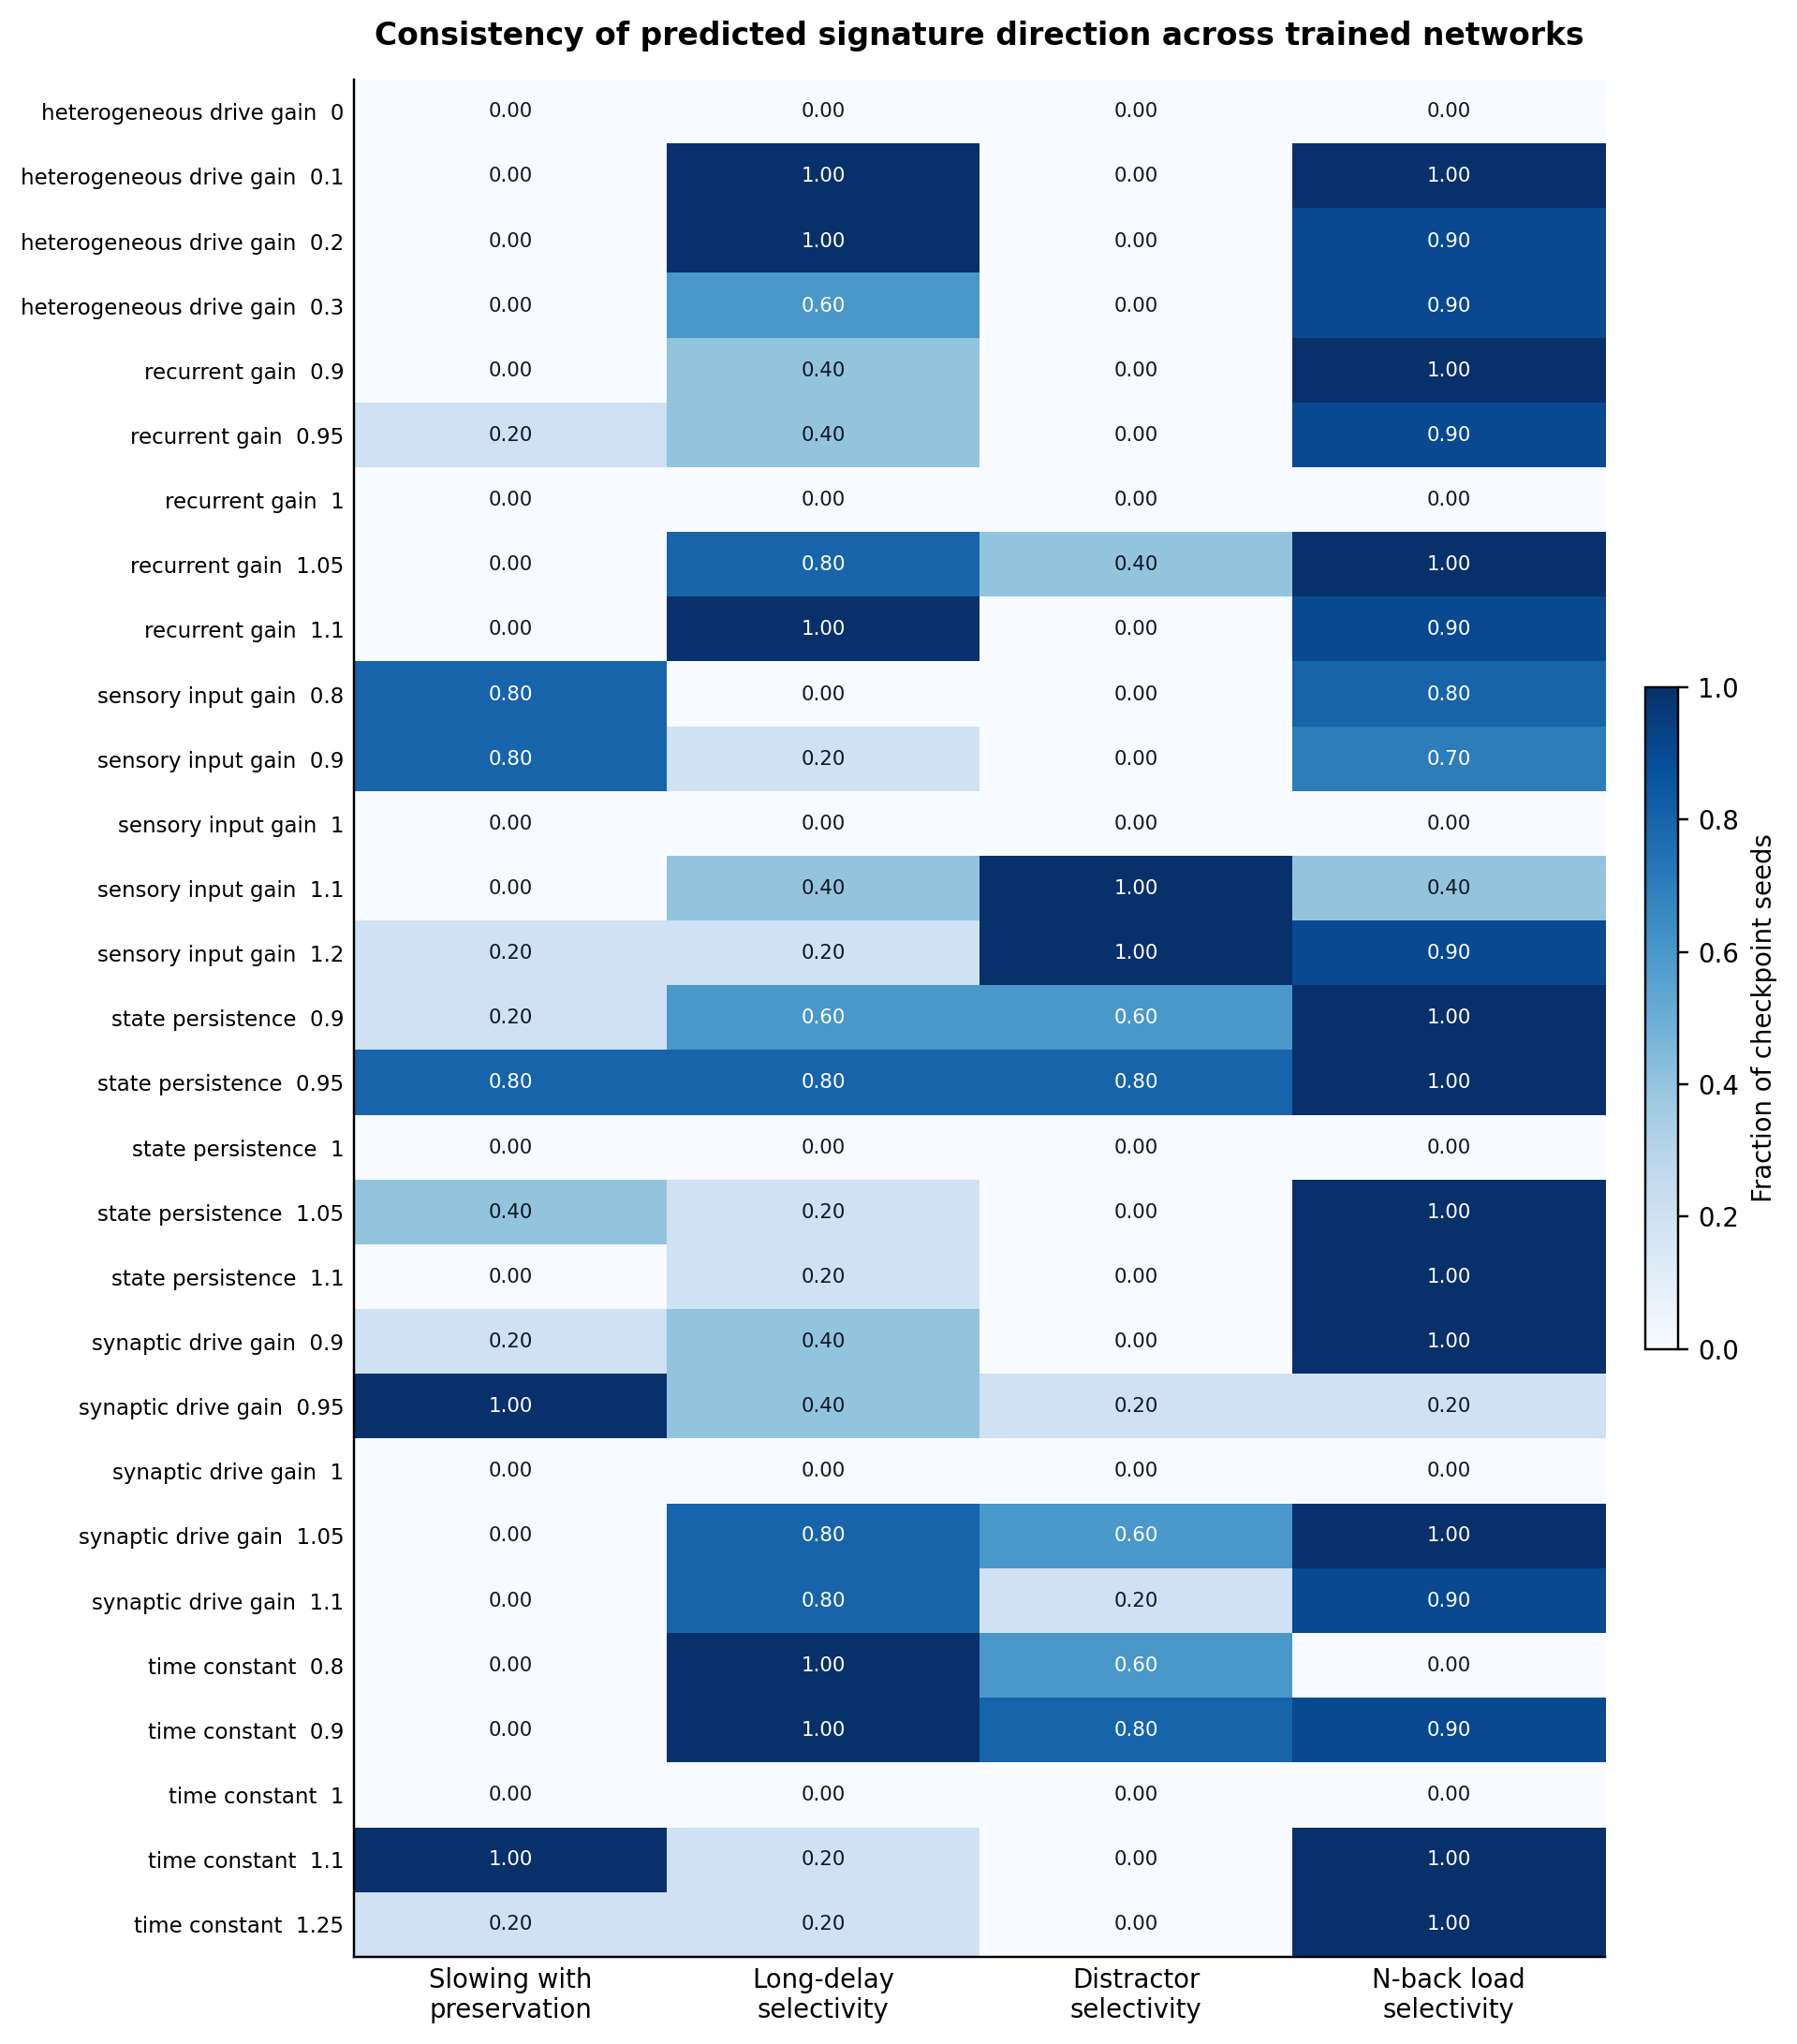
\includegraphics[height=0.72\textheight]{signature_screen.png}
  \caption{\textbf{Cross-task signature screen.}
  Rows are every shared operator-strength setting evaluated in both task
  families; columns show the fraction of independent checkpoint seeds with the
  predicted signature direction. Circular fractions have denominator five and
  N-back fractions denominator ten. State persistence 0.95 was the only row to
  meet the complete majority pattern and additionally reached 4/5 agreement on
  each circular feature with complete N-back agreement. Values quantify
  directional consistency, not participant-level probability or statistical
  significance.}
  \label{fig:screen}
\end{figure*}

\subsection{A 5\% persistence reduction preserved ordinary accuracy while
selectively affecting demanding conditions}

At $p=0.95$, clean delay-20 proportional angular-error change was
$0.049\pm0.092$ across circular checkpoints (95\% $t$-interval
$[-0.065,0.164]$) and remained below $0.20$ in 5/5 seeds. Restricted mean
settling increased by $0.104\pm0.167$ steps ($[-0.103,0.312]$) and was
positive in 4/5 seeds, with a range of $-0.013$ to $0.393$ steps
(Table~\ref{tab:leading}). The circular settling, delay, and distractor
intervals all include zero, so those components are directional majority
tendencies rather than robust across-checkpoint effects. By contrast, N-back
load selectivity was $0.250\pm0.077$ ($[0.195,0.305]$), positive in 10/10
checkpoints, and ranged from $0.110$ to $0.363$. Long-minus-short delay
selectivity was $0.089\pm0.075$ ($[-0.004,0.181]$) and distractor-minus-clean
selectivity was $0.015\pm0.044$ ($[-0.040,0.071]$), each positive in 4/5
checkpoints. Thus the leading perturbation retained the predicted average
ordering, but only the N-back contrast clearly excluded zero under the
seed-level $t$-interval.

\begin{table*}[t]
\caption{\textbf{State persistence 0.95.} Values are mean $\pm$ SD across five
circular or ten N-back checkpoint seeds; intervals are student $t$ 95\%
intervals across those seeds.}
\label{tab:leading}
\centering
\begin{tabular}{lccc}
\toprule
Outcome & Contrast & 95\% interval & Consistency \\
\midrule
Delay-20 error & $0.049\pm0.092$ & $[-0.065,0.164]$ & below 0.20 in 5/5 \\
Settling change (steps) & $0.104\pm0.167$ & $[-0.103,0.312]$ & 4/5 positive \\
Delay selectivity & $0.089\pm0.075$ & $[-0.004,0.181]$ & 4/5 positive \\
Distractor selectivity & $0.015\pm0.044$ & $[-0.040,0.071]$ & 4/5 positive \\
N-back load selectivity & $0.250\pm0.077$ & $[0.195,0.305]$ & 10/10 positive \\
\bottomrule
\end{tabular}
\end{table*}

\subsection{Persistence effects varied non-monotonically with perturbation
strength}

Reducing persistence further to 0.90 enlarged mean settling, delay, and N-back
load effects (Fig.~\ref{fig:persistence}). However, slowing with preservation
passed only 1/5 circular checkpoints, so the stronger intervention no longer
expressed the selective accuracy-preserving pattern. Increasing persistence
above one continued to impair N-back preferentially but reversed the circular
delay and distractor contrasts. The joint signature was therefore specific to
a weak reduction around 0.95 rather than monotonic damage at any non-neutral
strength.

\begin{figure*}[t]
  \centering
  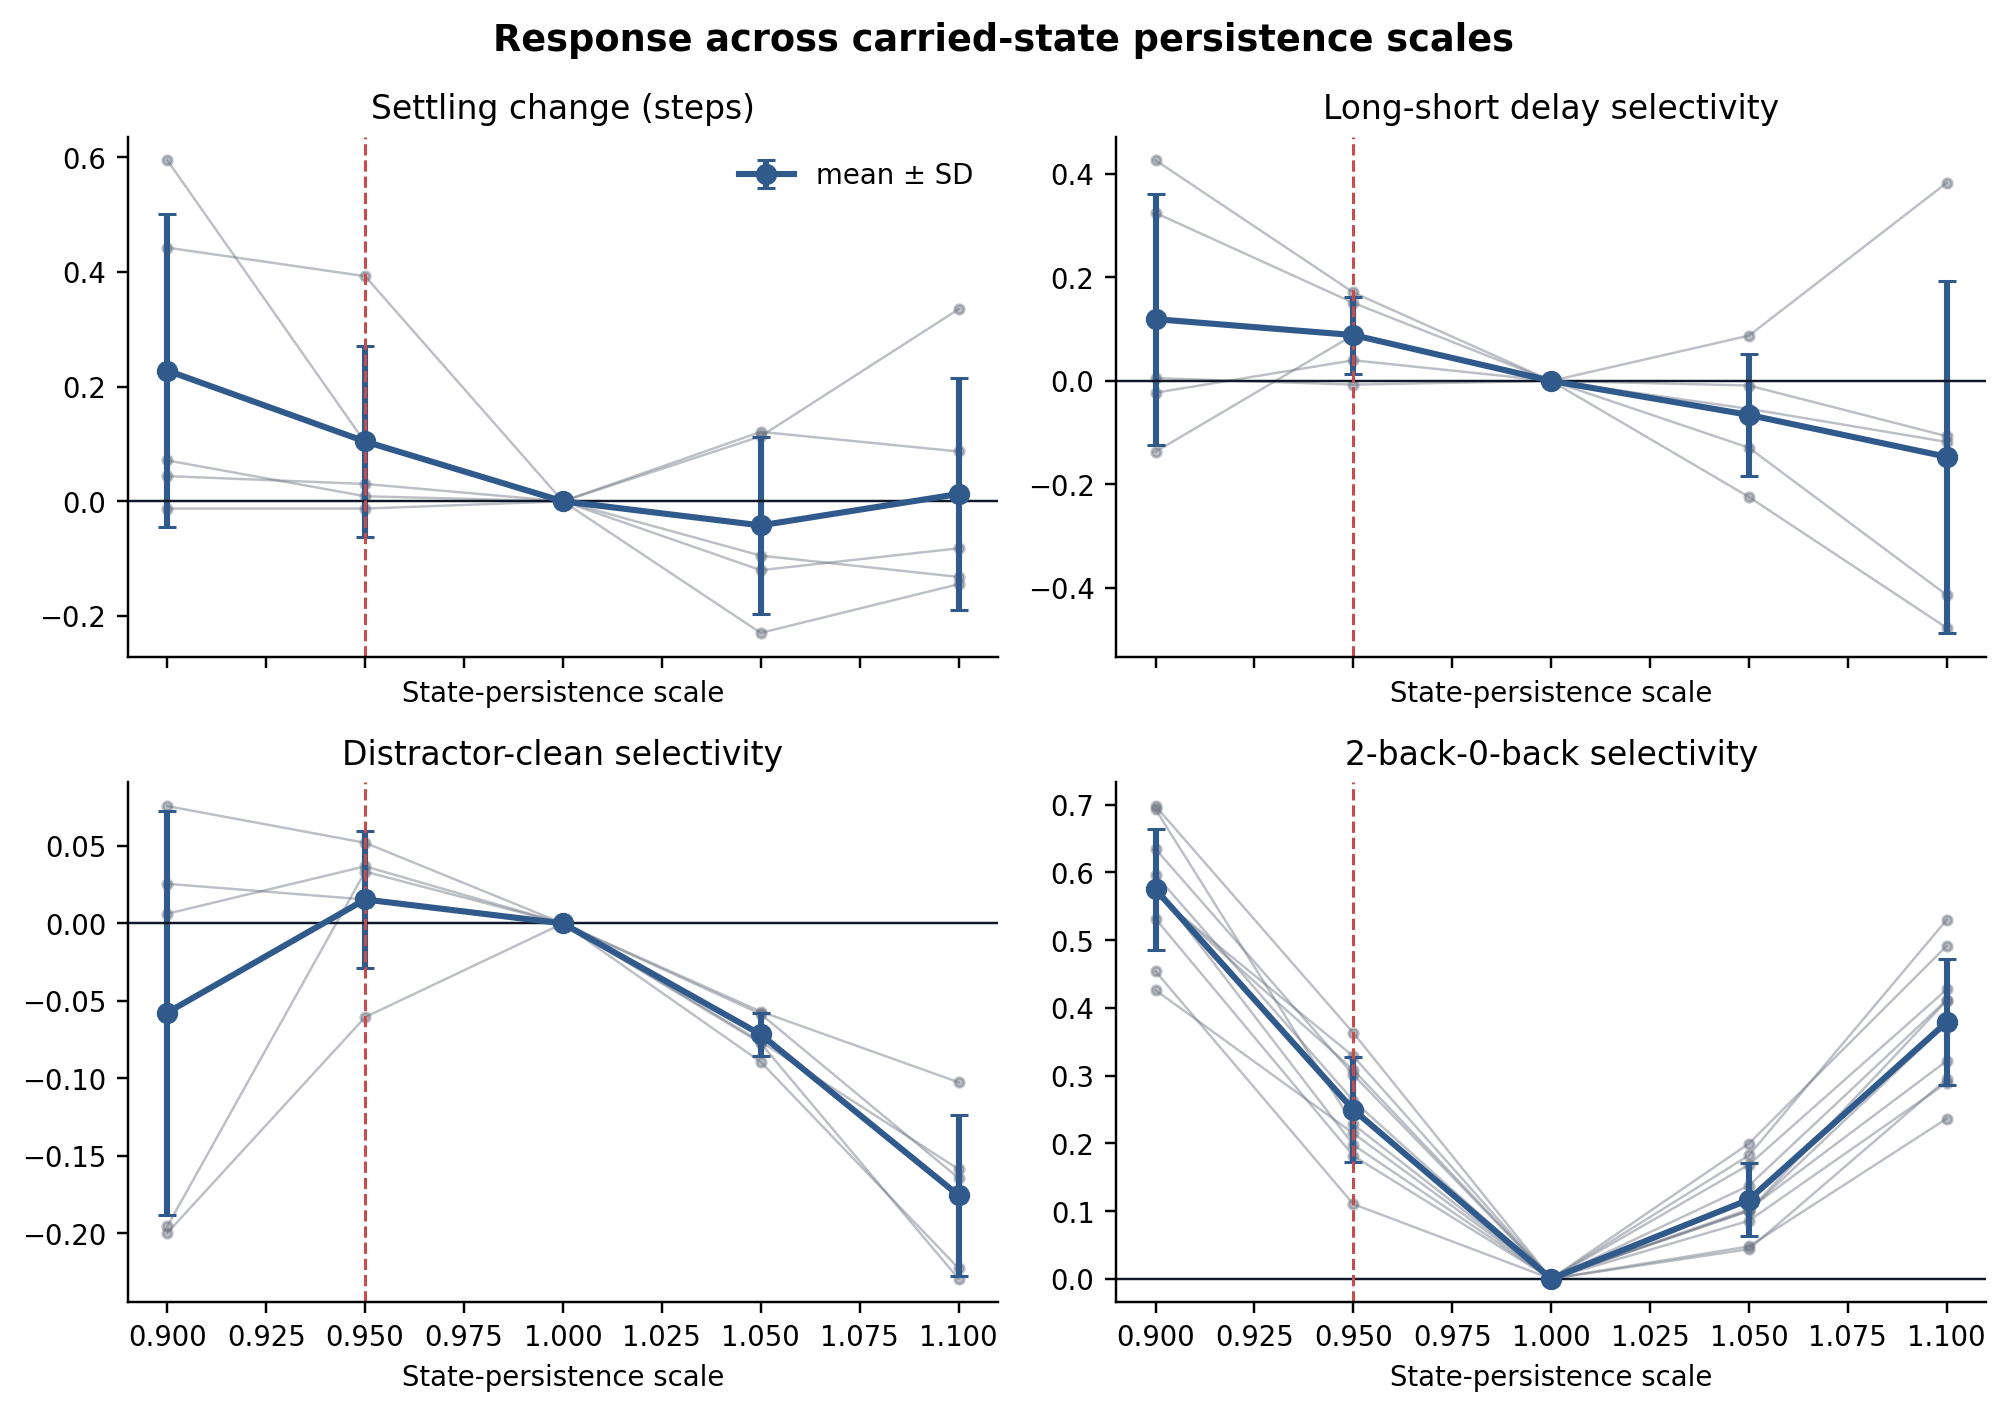
\includegraphics[width=0.98\textwidth]{persistence_dose_response.png}
  \caption{\textbf{Response across carried-state persistence scales.}
  The four panels report, from top-left to bottom-right: change in restricted
  mean settling steps, long-minus-short delay selectivity
  ($I_{\mathrm{delay\,80}}-I_{\mathrm{delay\,10}}$), distractor-minus-clean
  selectivity ($I_{\mathrm{distractor\,20}}-I_{\mathrm{clean\,20}}$), and
  2-back-minus-0-back load selectivity
  ($J_{\mathrm{2back}}-J_{\mathrm{0back}}$). Positive values indicate slower
  settling or larger impairment in the more demanding condition. Grey lines are
  independently trained checkpoint seeds; blue points and error bars are mean
  $\pm$ SD across seeds. The dashed red line marks the leading persistence scale
  0.95 and the horizontal line marks no change from each checkpoint's native
  baseline. A stronger reduction increased several impairments but also violated
  relative preservation, whereas increased persistence reversed circular delay
  and distractor selectivity.}
  \label{fig:persistence}
\end{figure*}

\subsection{Alternative operators reproduced partial signatures}

Sensory-input gain 1.20 produced distractor selectivity in 5/5 circular
checkpoints and load selectivity in 9/10 N-back checkpoints, but mean settling
became slightly faster ($-0.010\pm0.023$ steps; positive in only 1/5) and delay
selectivity was positive in only 1/5. Effective time-constant scale 1.10 slowed
settling with preservation in 5/5 ($0.605\pm0.176$ steps) and showed load
selectivity in 10/10, but distractor selectivity was negative in every circular
checkpoint. Conversely, time-constant scale 0.90 showed delay selectivity in
5/5 and distractor selectivity in 4/5 but accelerated settling in every
circular checkpoint ($-0.681\pm0.170$ steps). Synaptic-drive gain 1.05 showed
delay selectivity in 4/5, distractor selectivity in 3/5, and load selectivity
in 10/10, but also accelerated settling in 5/5 ($-0.496\pm0.240$ steps). All of
these near-miss clean delay-20 settling cells were latency-valid; uniqueness
was therefore not an artefact of invalid latency scoring. These near-misses
constrain the result: matching one difficult condition was insufficient to
qualify as the complete pattern, and the discrimination against the conserved
time-constant operator rested on settling direction and distractor selectivity
rather than on large absolute settling magnitude.

The contrast between persistence and the conserved time-constant operator is
mechanistically informative. Both reduced persistence ($p<1$) and reduced
timescale ($s<1$) can weaken retention, but only persistence leaves the drive
coefficient unchanged (Eq.~\ref{eq:persistence}). Reducing the conserved
timescale ($s=0.90$) accelerated post-cue settling while preserving delay and
distractor selectivity; increasing it ($s=1.10$) slowed settling but reversed
distractor selectivity. The joint pattern therefore depended on the asymmetric
carried-state intervention, not merely on any reduction in effective memory
lifetime. Cross-operator comparisons remain uncontrolled for overall clean-task
cost, so differences in perturbation magnitude could still contribute to some
near-misses.

\subsection{Native distractor competence and validity gates}

All 945 circular result rows passed the fixation gate, all ten N-back native
checkpoints passed competence, and all $p=0.95$ clean delay-20 cells were
latency-valid. Twelve rows elsewhere in the circular grid were latency-invalid
(all heterogeneous-drive settings with low settled fraction); none of the
near-miss settling comparisons above used those cells. Native distractor mean
error ranged from $3.46^\circ$ to $4.83^\circ$, and every native distractor cell
had a settled fraction of 1.00. The distractor contrast therefore measured
perturbation of a learned filtering behaviour rather than failure on an
unfamiliar task. As a manipulation check, distractor-window gains 1.10, 1.25,
and 1.50 increased distractor error by 3.7\%, 9.8\%, and 21.5\% on average,
respectively, with positive effects in 5/5 checkpoints. Persistence-related
distractor selectivity nevertheless remained small and was negative in one
checkpoint, so competent native filtering does not by itself make that contrast
a strong human effect-size match.

This screen did not include a matched-cost Gaussian comparator. Specificity
against generic disruption therefore remains an open next experiment rather
than a claim supported here.

\section{Discussion}

Reduced carried-state persistence was the only evaluated profile to meet the
complete descriptive majority rule for the selected cross-task behavioural
pattern against the native baseline. Scaling the carried-state coefficient by
0.95 left ordinary circular accuracy approximately intact while modestly
slowing response settling, increasing vulnerability at longer delays and under
distraction, and selectively impairing 2-back discriminability. The circular
components had the predicted mean signs and majority directional agreement,
but their seed-level intervals included zero; only the N-back load contrast was
robust across checkpoints.

Equation~\ref{eq:persistence} suggests a coherent model-level explanation.
Each update retains slightly less of the preceding hidden state without
simultaneously rescaling incoming drive. Information is therefore not erased
at once; rather, its stability is weakened cumulatively. Short and simple
conditions remain relatively intact, whereas longer maintenance, competing
input, and repeated updating expose the loss. The conserved time-constant
near-misses support this asymmetry reading: when carried-state and drive
coefficients are rescaled together, the joint signature breaks. The present
behavioural analyses do not directly demonstrate a changed attractor or slow
manifold.

Importantly, ``state persistence'' is an operational property of this
implemented recurrence, not a measured neurobiological parameter. Under the
descriptive scoring rule, the result shows candidate-versus-baseline qualitative
sufficiency: this intervention can generate the selected pattern. It does not
show that psilocybin reduces neural persistence, that 5-HT2A activation maps to
$p=0.95$, or that the mechanism is unique. A matched generic-damage comparator
remains the outstanding specificity test. Several alternative operators also
reproduced individual components. Subsequent analyses should therefore examine
hidden-state drift and stability and, separately, test specificity against
non-neutral matched-cost controls.

Two limitations particularly constrain the present inference. First, post-cue
settling is not literal reaction time because response onset was externally
imposed; moreover, the mean change was substantially less than one model step
and its across-seed interval included zero. Second, although the circular
networks were competent under distraction, the persistence distractor contrast
was only 0.015 on average, reversed in one checkpoint, and also had an interval
including zero. The circular delay contrast was likewise small
($0.089\pm0.075$). The circular task is also not the multiple-object tracking
paradigm used by Carter et al.\ \cite{carter2005}; it tests a related filtering
principle rather than reproducing that task. The descriptive grid contains
multiple operator-strength profiles but no confirmatory inferential family.
Checkpoint consistency demonstrates robustness across trained models, not
population inference about human participants.

The immediate next experiment should compare persistence $0.95$ with
matched-cost Gaussian disruption on these circular and N-back families, then
densify persistence scaling around 0.95 and quantify delay-period
representational drift on independently banked task samples. That specificity
analysis can retain the candidate-versus-baseline result reported here while
testing whether the pattern exceeds generic damage.

\section{Limitations and next steps for supervisor discussion}

\textbf{Key limitations to discuss.}
The central weakness is asymmetry across task families: N-back load selectivity
was robust, but circular delay and distractor selectivity were small and their
seed-level intervals included zero. The settling endpoint is also an imposed
model proxy rather than biological reaction time, and the observed slowing was
well below one model step on average. Mechanistic interpretation remains
behaviour-first: this report does not yet show whether persistence scaling
changes attractor geometry, manifold drift, or recovery dynamics in a way that
uniquely distinguishes it from other weak perturbations. Finally, the current
screen is candidate-versus-native only; without a matched-cost Gaussian
comparator, specificity against generic disruption remains untested.

\textbf{Immediate next steps.}
First, run the matched-cost Gaussian comparator on the same checkpoints and
banked samples, with preregistered cost matching to separate selective
signatures from generic damage. Second, densify persistence around 0.95 (for
example 0.93--0.98) to test whether the joint pattern is locally stable or a
narrow parameter point. Third, add targeted dynamics analyses on identical trials:
delay-period drift, local Jacobian spectrum near delay states, and perturbation
recovery trajectories after distractor input. Fourth, predefine a compact
confirmatory analysis family for the shortlisted contrasts so the next report
can move from descriptive directional consistency to controlled inferential
claims.

\section*{Conclusion}

A 5\% reduction in carried-state persistence was the only tested RNN
perturbation to reproduce the complete descriptive majority pattern on
distractor-trained circular networks and competence-screened N-back networks:
relative preservation with slower settling, greater long-delay and distractor
costs, and selective 2-back impairment. The circular pattern held in four of
five checkpoints and circular effect sizes were small, whereas N-back load
selectivity was robust across all ten checkpoints. Reduced persistence remains
a credible candidate for matched-cost specificity and mechanistic analysis, but
the present result is an abstract descriptive sufficiency finding against the
native baseline, not evidence for a biological mechanism of psilocybin.

\bibliographystyle{apsrev4-2}
\bibliography{full_candidate_perturbation_references}

\end{document}
